%%%%%%%%%%%%%%%%%%%%%%%%%%%%%%%%%%%%%%%%%
% Short Sectioned Assignment
% LaTeX Template
% Version 1.0 (5/5/12)
%
% This template has been downloaded from:
% http://www.LaTeXTemplates.com
%
% Original author:
% Frits Wenneker (http://www.howtotex.com)
%
% License:
% CC BY-NC-SA 3.0 (http://creativecommons.org/licenses/by-nc-sa/3.0/)
%
%%%%%%%%%%%%%%%%%%%%%%%%%%%%%%%%%%%%%%%%%

%----------------------------------------------------------------------------------------
%	PACKAGES AND OTHER DOCUMENT CONFIGURATIONS
%----------------------------------------------------------------------------------------

\documentclass[paper=a4, fontsize=11pt]{scrartcl} % A4 paper and 11pt font size

\usepackage[T1]{fontenc} % Use 8-bit encoding that has 256 glyphs
\usepackage[english]{babel} % English language/hyphenation
\usepackage{amsmath,amsfonts,amsthm} % Math packages


\usepackage{graphicx}
\usepackage{subfig}
\usepackage{amssymb}
\usepackage{hyperref}
\usepackage{float}


\usepackage{fancyhdr} % Custom headers and footers
\pagestyle{fancyplain} % Makes all pages in the document conform to the custom headers and footers
\fancyhead{} % No page header - if you want one, create it in the same way as the footers below
\fancyfoot[L]{} % Empty left footer
\fancyfoot[C]{} % Empty center footer
\fancyfoot[R]{\thepage} % Page numbering for right footer
\renewcommand{\headrulewidth}{0pt} % Remove header underlines
\renewcommand{\footrulewidth}{0pt} % Remove footer underlines
\setlength{\headheight}{6pt} % Customize the height of the header

\numberwithin{equation}{section} % Number equations within sections (i.e. 1.1, 1.2, 2.1, 2.2 instead of 1, 2, 3, 4)
\numberwithin{figure}{section} % Number figures within sections (i.e. 1.1, 1.2, 2.1, 2.2 instead of 1, 2, 3, 4)
\numberwithin{table}{section} % Number tables within sections (i.e. 1.1, 1.2, 2.1, 2.2 instead of 1, 2, 3, 4)

\setlength\parindent{0pt} % Removes all indentation from paragraphs - comment this line for an assignment with lots of text

%----------------------------------------------------------------------------------------
%	TITLE SECTION
%----------------------------------------------------------------------------------------

\newcommand{\horrule}[1]{\rule{\linewidth}{#1}} % Create horizontal rule command with 1 argument of height

\title{	
\normalfont \normalsize 
\textsc{UC Berkeley, Computer Science} \\ [25pt] % Your university, school and/or department name(s)
\horrule{0.5pt} \\[0.4cm] % Thin top horizontal rule
\huge CS289A Project Proposal \\ % The assignment title
\horrule{2pt} \\[0.5cm] % Thick bottom horizontal rule
}

\author{Peter Cheng, Jeff Tsui, Alice Wang} % Your name

\date{\normalsize\today} % Today's date or a custom date

\begin{document}

\maketitle % Print the title

\section{Overview}
Our project will be to design and test an off-line classifier for
gender prediction from handwritten text. The inspiration for this
project is from a recent machine learning competition hosted on
Kaggle, a website which often runs such contests\cite{kaggle}. Kaggle
provides sample training and testing data, in the form of
high-resolution jpg images. Each image corresponds to a writing
sample, and there are 4 writing samples for each of 475 writers. The 4
samples correspond to:

\begin{enumerate}
\item Arabic text, different text for each writer
\item Arabic text, same text for each writer
\item English text, different text for each writer
\item English text, same text for each writer
\end{enumerate}

Kaggle also provides extracted features for each writing sample, using
methods described in \cite{geometricFeatures}. An example of an image sample is shown in Figure \ref{fig:sample}.

\section{Approach}
The Kaggle competition page provides references to a number of
relevant papers for extracting features from writing samples and
constructing classifiers. From a preliminary scan through related
literature, it appears that acquiring strong features is as important,
if not more important than the construction of models for
classification. We have also come across numerous papers describing
different types of features, and the design of such features appears
to be a very interesting problem. As a result, we are currently opting
to generate features ourselves, and have begun implementing and
testing methods encountered during our literature search. We also will
have to perform a number of preprocessing steps, as the Kaggle dataset
is highly unconstrained. The images contain color and some amount of
noise, the handwriting is not centered, and much of the text is
written at a curve or a slant. As a result, segmenting and extracting
lines, words, and characters from each image will be a challenge in
itself, and this needs to be performed before a large number of
features can be acquired. Once we have successfully extracted features
from our images, we should be able to implement the numerous
classifiers we have learned from class, and benchmark our results
against those obtained by the sources we are borrowing from.

\begin{figure}
  \centering \fbox{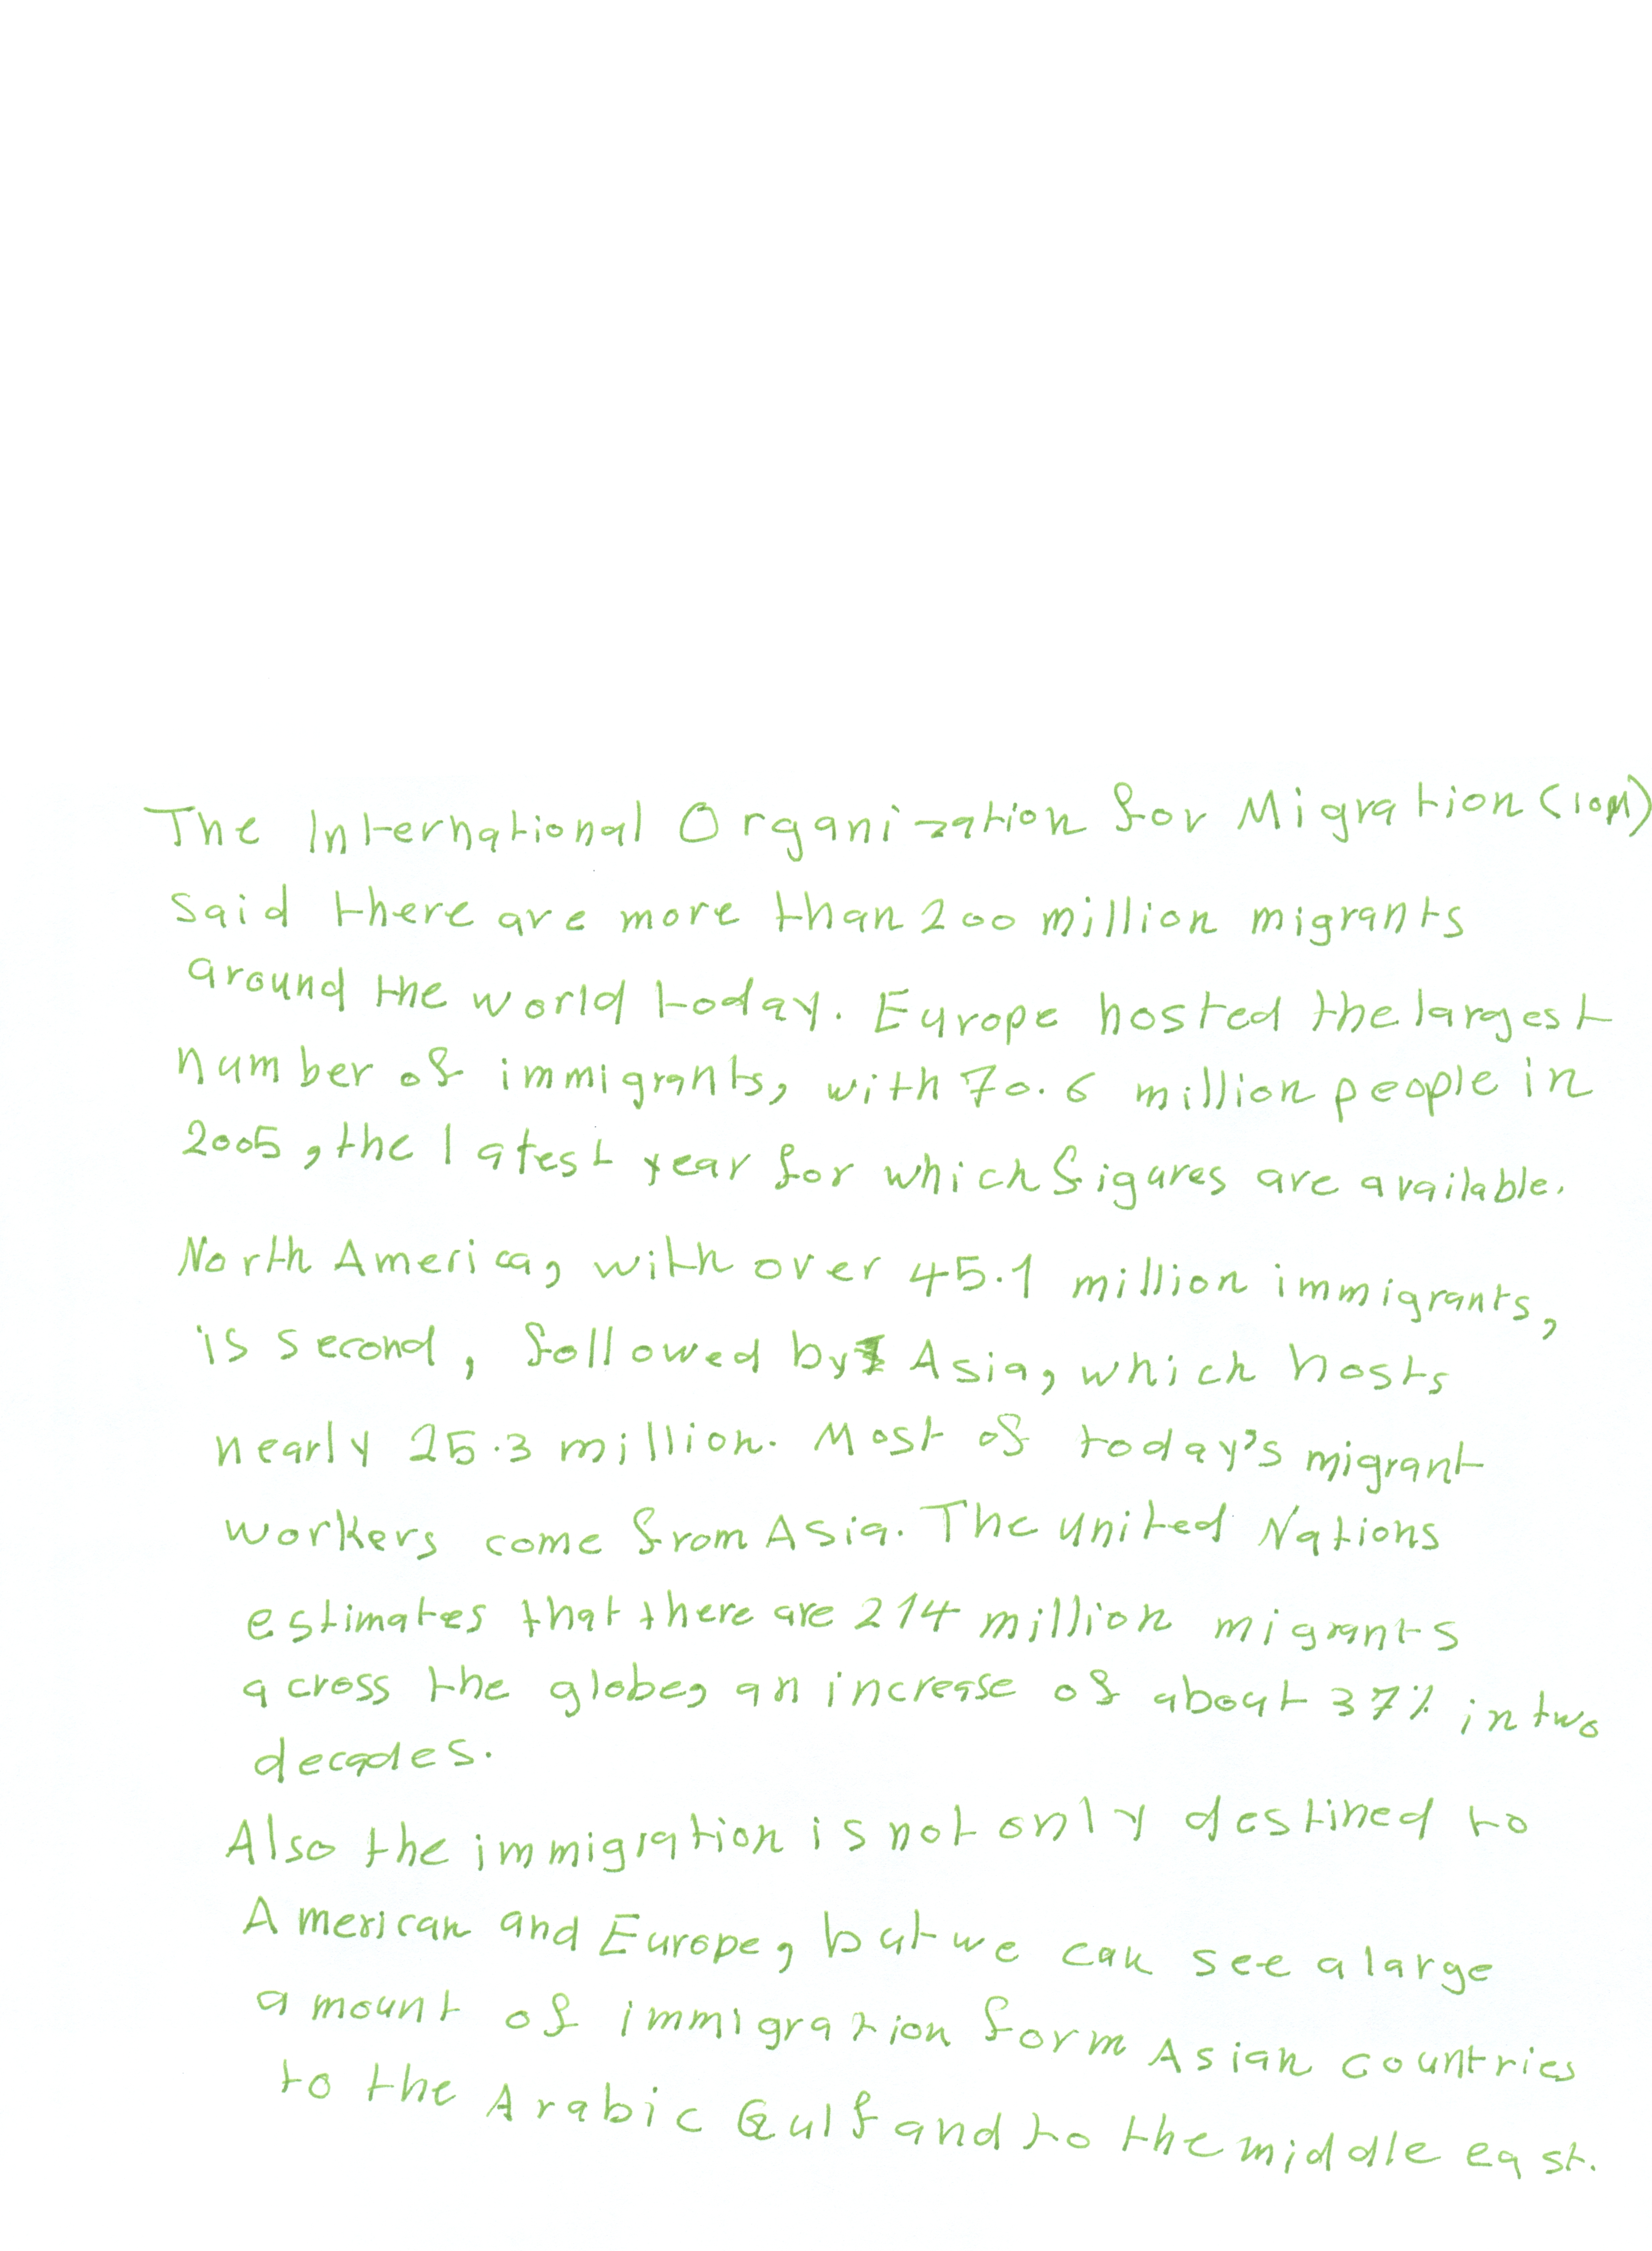
\includegraphics[width=2.6in]{im.jpg}}
  \caption{A sample training image\\}
  \label{fig:sample}
\end{figure}

\bibliography{report} %>>>> bibliography data in report.bib
\bibliographystyle{spiebib} %>>>> makes bibtex use spiebib.bst

\end{document}